\documentclass{article}
\usepackage[utf8]{inputenc}
\usepackage[T1]{fontenc}
\usepackage[francais]{babel}
\usepackage{lmodern}
\usepackage{graphicx}
\usepackage{geometry}
\usepackage{tikz}

\geometry{hmargin=30pt, vmargin=30pt}

\title{Schéma global du projet : Tableau virtuel interactif}
\author{Bollini Kevin, Mélia Geoffrey, Pagès Julien, Saleil Baptiste}

\begin{document}

\maketitle

\section{Introduction}
Avant propos : Ce document présente notre projet et donne un aperçu du fonctionnement de notre application.
\paragraph{}
Le but de l’application est de simuler une écriture ou un dessin sur un tableau virtuel. Ceci en se basant sur une
reconnaissance de mouvements via une webcam. Le projet comporte deux parties distinctes : 
la librairie -que nous nommeront libtrack- permettant de réaliser le suivi des objets dans le flux vidéo acquis par la webcam ; et l'application proposant une interface graphique permettant à un ou plusieurs utilisateurs de dessiner.

\begin{figure}[h]
\begin{center}
	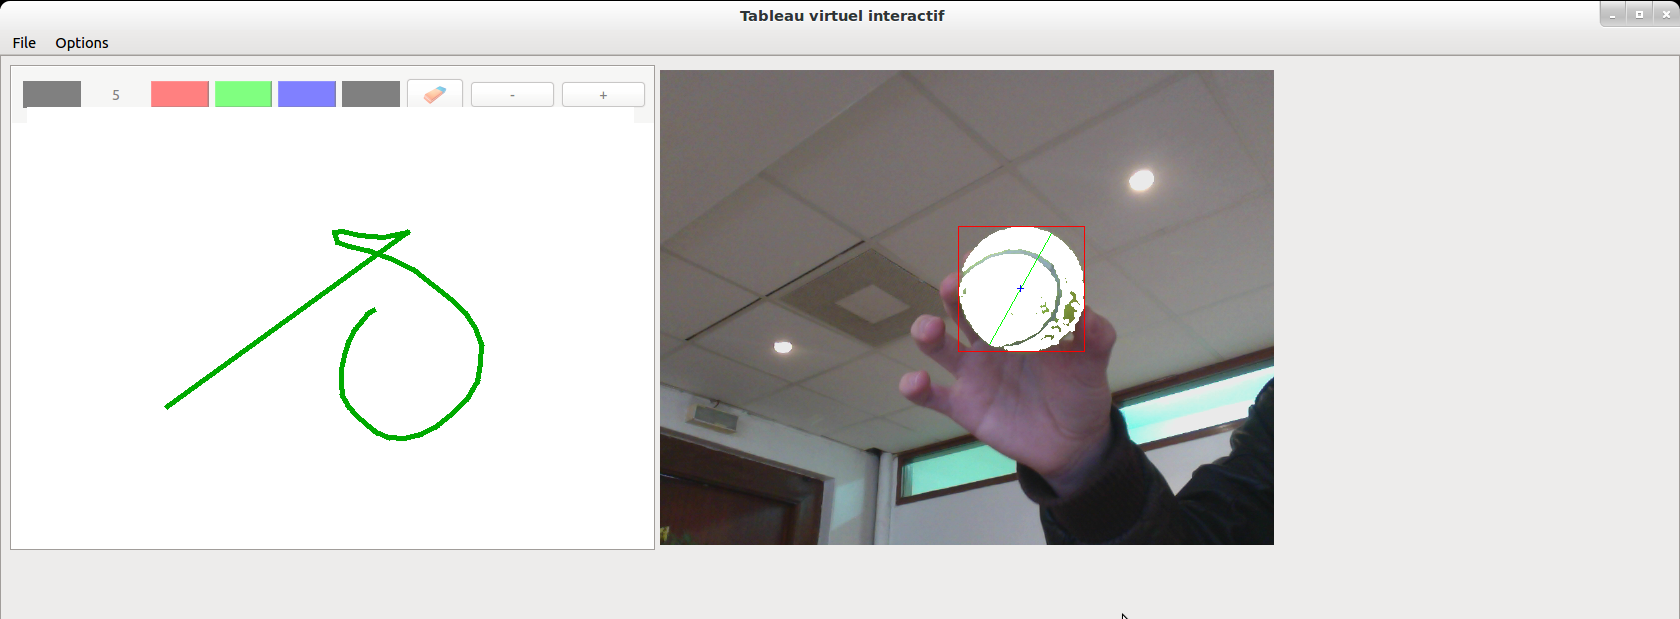
\includegraphics[scale=0.4]{capture.png}
	\caption{Utilisation du logiciel}
\end{center}
\end{figure}

\section{Schéma Global}
Le schéma ci dessous présente de façon globale les différents modules pour une utilisation en réseau de l'application.
	\begin{figure}[h]
	\begin{center}
	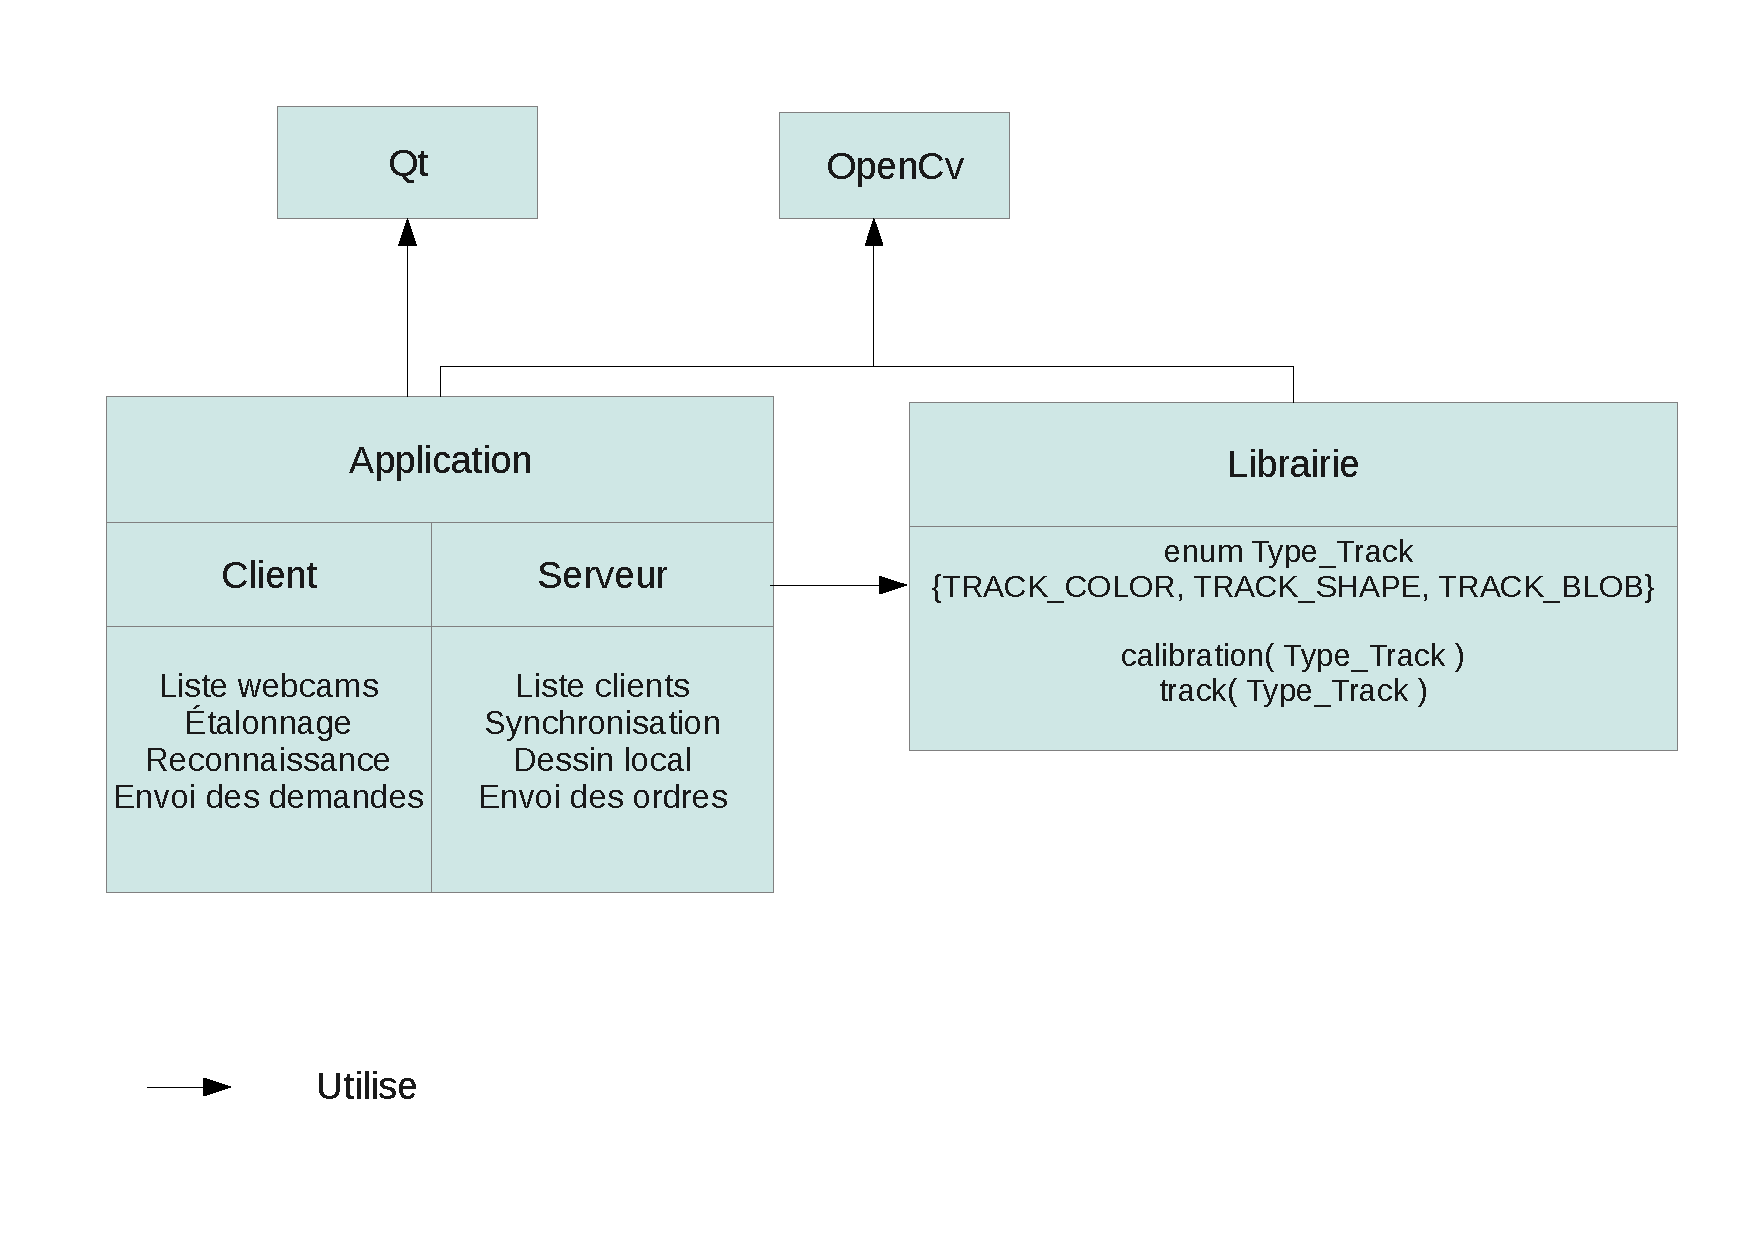
\includegraphics[scale=0.5]{schema_global.pdf}
	\caption{Différents modules du projet}
	\end{center}
	\end{figure}
Le client et le serveur sont écrits à l'aide de la librairie Qt. Le client fait appel à la librairie libtrack pour reconnaître les mouvements. \\
Cette dernière utilise OpenCV pour le traitement de l'image et se veut réutilisable d pour'autres projets. 
Elle contient principalement une fonction d'étalonnage qui permet de signifier l'objet à suivre, ainsi que le type de suivi (Couleur, forme, avec cvBlob). La librairie possède ensuite un seul point d'entrée permettant d'effectuer le suivi.

\newpage
\section{Architecture de l'application}
L'application est conçue entièrement par dessus la librairie en essayant de minimimer le nombre de fonctions appelées. 
L'étalonnage du suivi de l'objet est effectué dans la classe $Calibration$, ensuite les appels pour suivre les mouvements sont faits
via une seule fonction dans la classe $WidgetWebcam$ qui transmets ses mouvements au $Client$ (classe principale). \\

De plus l'application est conçue pour fonctionner de manière similaire pour une utilisation en réseau, ou en local, les classes 
représentant le tableau en local ou en réseau ont donc la même apparence (mêmes points d'entrées) vu de l'extérieur. \\
	\begin{center}
		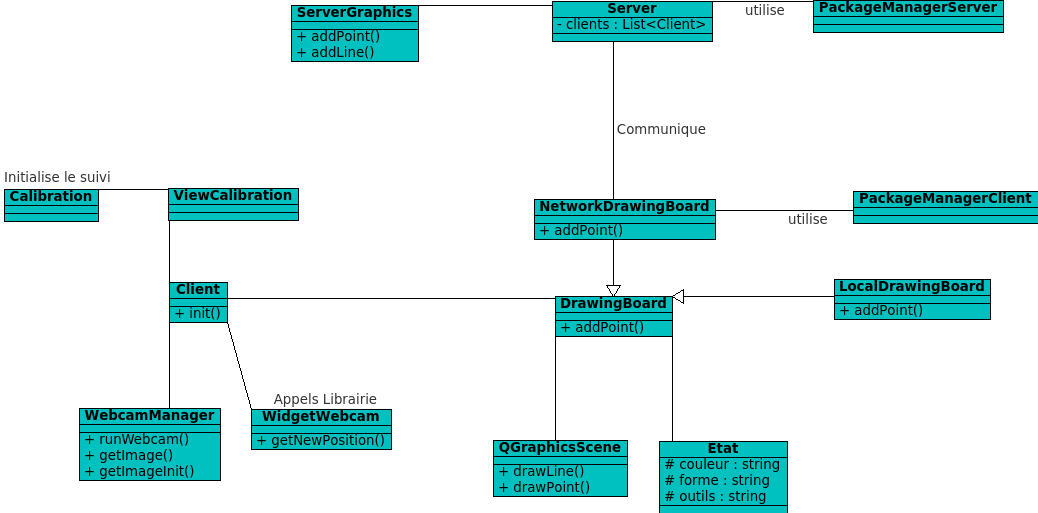
\includegraphics[scale=0.7]{../uml/classes.png}
	\end{center}

\section{Schéma lors d'une utilisation en réseau}
Ce schéma présente un déroulement des opérations lors d'une connexion et d'un dessin en utilisant les fonctionnalités réseaux.\\

\begin{itemize}
	\item Le client se connecte
	\item Le client effectue son étalonnage
	\item Le serveur l'enregistre, et lui envoie le tableau courant (vide ou non)
	\item Le client stocke le tableau et commence à détecter un mouvement
	\item Il envoie le mouvement détecté
	\item Le serveur reçoit le mouvement, dessine en local et renvoie à tous les clients l'ordre de dessin
	\item Le client reçoit l'ordre et dessine en local
\end{itemize}

\begin{figure}[h]
	\begin{center}
		% Graphic for TeX using PGF
% Title: /home/julien/master/projet/dessin-realite-augmentee/documents/uml/sequence_reseau.dia
% Creator: Dia v0.97.2
% CreationDate: Tue Apr 24 10:47:45 2012
% For: julien
% \usepackage{tikz}
% The following commands are not supported in PSTricks at present
% We define them conditionally, so when they are implemented,
% this pgf file will use them.
\ifx\du\undefined
  \newlength{\du}
\fi
\setlength{\du}{15\unitlength}
\begin{tikzpicture}
\pgftransformxscale{1.000000}
\pgftransformyscale{-1.000000}
\definecolor{dialinecolor}{rgb}{0.000000, 0.000000, 0.000000}
\pgfsetstrokecolor{dialinecolor}
\definecolor{dialinecolor}{rgb}{1.000000, 1.000000, 1.000000}
\pgfsetfillcolor{dialinecolor}
\pgfsetlinewidth{0.100000\du}
\pgfsetdash{}{0pt}
\definecolor{dialinecolor}{rgb}{1.000000, 1.000000, 1.000000}
\pgfsetfillcolor{dialinecolor}
\fill (5.000000\du,7.000000\du)--(5.000000\du,8.400000\du)--(9.042500\du,8.400000\du)--(9.042500\du,7.000000\du)--cycle;
\definecolor{dialinecolor}{rgb}{0.000000, 0.000000, 0.000000}
\pgfsetstrokecolor{dialinecolor}
\draw (5.000000\du,7.000000\du)--(5.000000\du,8.400000\du)--(9.042500\du,8.400000\du)--(9.042500\du,7.000000\du)--cycle;
% setfont left to latex
\definecolor{dialinecolor}{rgb}{0.000000, 0.000000, 0.000000}
\pgfsetstrokecolor{dialinecolor}
\node at (7.021250\du,7.950000\du){Serveur};
\definecolor{dialinecolor}{rgb}{1.000000, 1.000000, 1.000000}
\pgfsetfillcolor{dialinecolor}
\fill (5.000000\du,8.400000\du)--(5.000000\du,8.800000\du)--(9.042500\du,8.800000\du)--(9.042500\du,8.400000\du)--cycle;
\definecolor{dialinecolor}{rgb}{0.000000, 0.000000, 0.000000}
\pgfsetstrokecolor{dialinecolor}
\draw (5.000000\du,8.400000\du)--(5.000000\du,8.800000\du)--(9.042500\du,8.800000\du)--(9.042500\du,8.400000\du)--cycle;
\definecolor{dialinecolor}{rgb}{1.000000, 1.000000, 1.000000}
\pgfsetfillcolor{dialinecolor}
\fill (5.000000\du,8.800000\du)--(5.000000\du,9.200000\du)--(9.042500\du,9.200000\du)--(9.042500\du,8.800000\du)--cycle;
\definecolor{dialinecolor}{rgb}{0.000000, 0.000000, 0.000000}
\pgfsetstrokecolor{dialinecolor}
\draw (5.000000\du,8.800000\du)--(5.000000\du,9.200000\du)--(9.042500\du,9.200000\du)--(9.042500\du,8.800000\du)--cycle;
\pgfsetlinewidth{0.100000\du}
\pgfsetdash{}{0pt}
\definecolor{dialinecolor}{rgb}{1.000000, 1.000000, 1.000000}
\pgfsetfillcolor{dialinecolor}
\fill (27.000000\du,7.000000\du)--(27.000000\du,8.400000\du)--(30.132500\du,8.400000\du)--(30.132500\du,7.000000\du)--cycle;
\definecolor{dialinecolor}{rgb}{0.000000, 0.000000, 0.000000}
\pgfsetstrokecolor{dialinecolor}
\draw (27.000000\du,7.000000\du)--(27.000000\du,8.400000\du)--(30.132500\du,8.400000\du)--(30.132500\du,7.000000\du)--cycle;
% setfont left to latex
\definecolor{dialinecolor}{rgb}{0.000000, 0.000000, 0.000000}
\pgfsetstrokecolor{dialinecolor}
\node at (28.566250\du,7.950000\du){Client};
\definecolor{dialinecolor}{rgb}{1.000000, 1.000000, 1.000000}
\pgfsetfillcolor{dialinecolor}
\fill (27.000000\du,8.400000\du)--(27.000000\du,8.800000\du)--(30.132500\du,8.800000\du)--(30.132500\du,8.400000\du)--cycle;
\definecolor{dialinecolor}{rgb}{0.000000, 0.000000, 0.000000}
\pgfsetstrokecolor{dialinecolor}
\draw (27.000000\du,8.400000\du)--(27.000000\du,8.800000\du)--(30.132500\du,8.800000\du)--(30.132500\du,8.400000\du)--cycle;
\definecolor{dialinecolor}{rgb}{1.000000, 1.000000, 1.000000}
\pgfsetfillcolor{dialinecolor}
\fill (27.000000\du,8.800000\du)--(27.000000\du,9.200000\du)--(30.132500\du,9.200000\du)--(30.132500\du,8.800000\du)--cycle;
\definecolor{dialinecolor}{rgb}{0.000000, 0.000000, 0.000000}
\pgfsetstrokecolor{dialinecolor}
\draw (27.000000\du,8.800000\du)--(27.000000\du,9.200000\du)--(30.132500\du,9.200000\du)--(30.132500\du,8.800000\du)--cycle;
\pgfsetlinewidth{0.050000\du}
\pgfsetdash{}{0pt}
\pgfsetdash{{0.400000\du}{0.400000\du}}{0\du}
\definecolor{dialinecolor}{rgb}{0.000000, 0.000000, 0.000000}
\pgfsetstrokecolor{dialinecolor}
\draw (29.000000\du,8.000000\du)--(29.000000\du,28.000000\du);
\definecolor{dialinecolor}{rgb}{0.000000, 0.000000, 0.000000}
\pgfsetstrokecolor{dialinecolor}
\draw (29.000000\du,30.000000\du)--(29.000000\du,31.000000\du);
\pgfsetlinewidth{0.100000\du}
\pgfsetdash{}{0pt}
\definecolor{dialinecolor}{rgb}{1.000000, 1.000000, 1.000000}
\pgfsetfillcolor{dialinecolor}
\fill (28.650000\du,28.000000\du)--(28.650000\du,30.000000\du)--(29.350000\du,30.000000\du)--(29.350000\du,28.000000\du)--cycle;
\definecolor{dialinecolor}{rgb}{0.000000, 0.000000, 0.000000}
\pgfsetstrokecolor{dialinecolor}
\draw (28.650000\du,28.000000\du)--(28.650000\du,30.000000\du)--(29.350000\du,30.000000\du)--(29.350000\du,28.000000\du)--cycle;
\pgfsetlinewidth{0.050000\du}
\pgfsetdash{}{0pt}
\pgfsetdash{{0.400000\du}{0.400000\du}}{0\du}
\definecolor{dialinecolor}{rgb}{0.000000, 0.000000, 0.000000}
\pgfsetstrokecolor{dialinecolor}
\draw (7.021250\du,8.100000\du)--(7.021250\du,28.000000\du);
\definecolor{dialinecolor}{rgb}{0.000000, 0.000000, 0.000000}
\pgfsetstrokecolor{dialinecolor}
\draw (7.021250\du,30.000000\du)--(7.021250\du,31.000000\du);
\pgfsetlinewidth{0.100000\du}
\pgfsetdash{}{0pt}
\definecolor{dialinecolor}{rgb}{1.000000, 1.000000, 1.000000}
\pgfsetfillcolor{dialinecolor}
\fill (6.671250\du,28.000000\du)--(6.671250\du,30.000000\du)--(7.371250\du,30.000000\du)--(7.371250\du,28.000000\du)--cycle;
\definecolor{dialinecolor}{rgb}{0.000000, 0.000000, 0.000000}
\pgfsetstrokecolor{dialinecolor}
\draw (6.671250\du,28.000000\du)--(6.671250\du,30.000000\du)--(7.371250\du,30.000000\du)--(7.371250\du,28.000000\du)--cycle;
\pgfsetlinewidth{0.100000\du}
\pgfsetbuttcap
\pgfsetdash{}{0pt}
{
\definecolor{dialinecolor}{rgb}{0.000000, 0.000000, 0.000000}
\pgfsetfillcolor{dialinecolor}
% was here!!!
\pgfsetarrowsstart{latex}
\definecolor{dialinecolor}{rgb}{0.000000, 0.000000, 0.000000}
\pgfsetstrokecolor{dialinecolor}
\draw (7.050000\du,11.850000\du)--(28.900000\du,11.850000\du);
}
% setfont left to latex
\definecolor{dialinecolor}{rgb}{0.000000, 0.000000, 0.000000}
\pgfsetstrokecolor{dialinecolor}
\node at (18.250000\du,11.300000\du){Connexion};
\pgfsetlinewidth{0.100000\du}
\pgfsetdash{}{0pt}
\pgfsetdash{}{0pt}
\pgfsetbuttcap
{
\definecolor{dialinecolor}{rgb}{0.000000, 0.000000, 0.000000}
\pgfsetfillcolor{dialinecolor}
% was here!!!
\pgfsetarrowsend{stealth}
\definecolor{dialinecolor}{rgb}{0.000000, 0.000000, 0.000000}
\pgfsetstrokecolor{dialinecolor}
\draw (7.100000\du,11.900000\du)--(7.150000\du,14.550000\du);
}
\pgfsetlinewidth{0.100000\du}
\pgfsetbuttcap
\pgfsetdash{}{0pt}
{
\definecolor{dialinecolor}{rgb}{0.000000, 0.000000, 0.000000}
\pgfsetfillcolor{dialinecolor}
% was here!!!
\pgfsetarrowsstart{latex}
\definecolor{dialinecolor}{rgb}{0.000000, 0.000000, 0.000000}
\pgfsetstrokecolor{dialinecolor}
\draw (28.950000\du,14.700000\du)--(7.200000\du,14.650000\du);
}
% setfont left to latex
\definecolor{dialinecolor}{rgb}{0.000000, 0.000000, 0.000000}
\pgfsetstrokecolor{dialinecolor}
\node at (17.850000\du,14.300000\du){Envoi tableau};
% setfont left to latex
\definecolor{dialinecolor}{rgb}{0.000000, 0.000000, 0.000000}
\pgfsetstrokecolor{dialinecolor}
\node[anchor=west] at (27.000000\du,11.000000\du){Étalonnage};
% setfont left to latex
\definecolor{dialinecolor}{rgb}{0.000000, 0.000000, 0.000000}
\pgfsetstrokecolor{dialinecolor}
\node[anchor=west] at (2.750000\du,12.950000\du){Stockage du };
% setfont left to latex
\definecolor{dialinecolor}{rgb}{0.000000, 0.000000, 0.000000}
\pgfsetstrokecolor{dialinecolor}
\node[anchor=west] at (2.750000\du,13.750000\du){client};
\pgfsetlinewidth{0.100000\du}
\pgfsetbuttcap
\pgfsetdash{}{0pt}
{
\definecolor{dialinecolor}{rgb}{0.000000, 0.000000, 0.000000}
\pgfsetfillcolor{dialinecolor}
% was here!!!
\pgfsetarrowsstart{latex}
\definecolor{dialinecolor}{rgb}{0.000000, 0.000000, 0.000000}
\pgfsetstrokecolor{dialinecolor}
\draw (28.900000\du,17.250000\du)--(29.000000\du,14.800000\du);
}
% setfont left to latex
% setfont left to latex
\definecolor{dialinecolor}{rgb}{0.000000, 0.000000, 0.000000}
\pgfsetstrokecolor{dialinecolor}
\node[anchor=west] at (29.600000\du,15.900000\du){Stocke le tableau reçu};
% setfont left to latex
\definecolor{dialinecolor}{rgb}{0.000000, 0.000000, 0.000000}
\pgfsetstrokecolor{dialinecolor}
\node[anchor=west] at (29.600000\du,16.700000\du){en local};
\pgfsetlinewidth{0.100000\du}
\pgfsetbuttcap
\pgfsetdash{}{0pt}
{
\definecolor{dialinecolor}{rgb}{0.000000, 0.000000, 0.000000}
\pgfsetfillcolor{dialinecolor}
% was here!!!
\pgfsetarrowsstart{latex}
\definecolor{dialinecolor}{rgb}{0.000000, 0.000000, 0.000000}
\pgfsetstrokecolor{dialinecolor}
\draw (7.050000\du,19.450000\du)--(28.850000\du,19.450000\du);
}
% setfont left to latex
\definecolor{dialinecolor}{rgb}{0.000000, 0.000000, 0.000000}
\pgfsetstrokecolor{dialinecolor}
\node at (17.950000\du,19.950000\du){Mouvement(x, y)};
% setfont left to latex
\definecolor{dialinecolor}{rgb}{0.000000, 0.000000, 0.000000}
\pgfsetstrokecolor{dialinecolor}
\node[anchor=west] at (2.850000\du,20.200000\du){Réception };
% setfont left to latex
\definecolor{dialinecolor}{rgb}{0.000000, 0.000000, 0.000000}
\pgfsetstrokecolor{dialinecolor}
\node[anchor=west] at (2.850000\du,21.000000\du){du message};
% setfont left to latex
\definecolor{dialinecolor}{rgb}{0.000000, 0.000000, 0.000000}
\pgfsetstrokecolor{dialinecolor}
\node[anchor=west] at (2.900000\du,22.350000\du){Dessin en};
% setfont left to latex
\definecolor{dialinecolor}{rgb}{0.000000, 0.000000, 0.000000}
\pgfsetstrokecolor{dialinecolor}
\node[anchor=west] at (2.900000\du,23.150000\du){local};
\pgfsetlinewidth{0.100000\du}
\pgfsetbuttcap
\pgfsetdash{}{0pt}
{
\definecolor{dialinecolor}{rgb}{0.000000, 0.000000, 0.000000}
\pgfsetfillcolor{dialinecolor}
% was here!!!
\pgfsetarrowsstart{latex}
\definecolor{dialinecolor}{rgb}{0.000000, 0.000000, 0.000000}
\pgfsetstrokecolor{dialinecolor}
\draw (7.150000\du,21.800000\du)--(7.150000\du,19.550000\du);
}
% setfont left to latex
\pgfsetlinewidth{0.100000\du}
\pgfsetbuttcap
\pgfsetdash{}{0pt}
{
\definecolor{dialinecolor}{rgb}{0.000000, 0.000000, 0.000000}
\pgfsetfillcolor{dialinecolor}
% was here!!!
\pgfsetarrowsstart{latex}
\definecolor{dialinecolor}{rgb}{0.000000, 0.000000, 0.000000}
\pgfsetstrokecolor{dialinecolor}
\draw (7.150000\du,23.700000\du)--(7.150000\du,21.800000\du);
}
% setfont left to latex
\pgfsetlinewidth{0.100000\du}
\pgfsetbuttcap
\pgfsetdash{}{0pt}
{
\definecolor{dialinecolor}{rgb}{0.000000, 0.000000, 0.000000}
\pgfsetfillcolor{dialinecolor}
% was here!!!
\pgfsetarrowsstart{latex}
\definecolor{dialinecolor}{rgb}{0.000000, 0.000000, 0.000000}
\pgfsetstrokecolor{dialinecolor}
\draw (28.950000\du,19.450000\du)--(28.950000\du,17.150000\du);
}
% setfont left to latex
% setfont left to latex
\definecolor{dialinecolor}{rgb}{0.000000, 0.000000, 0.000000}
\pgfsetstrokecolor{dialinecolor}
\node[anchor=west] at (29.650000\du,18.100000\du){Détecte les mouvements};
\pgfsetlinewidth{0.100000\du}
\pgfsetbuttcap
\pgfsetdash{}{0pt}
{
\definecolor{dialinecolor}{rgb}{0.000000, 0.000000, 0.000000}
\pgfsetfillcolor{dialinecolor}
% was here!!!
\pgfsetarrowsstart{latex}
\definecolor{dialinecolor}{rgb}{0.000000, 0.000000, 0.000000}
\pgfsetstrokecolor{dialinecolor}
\draw (29.000000\du,24.000000\du)--(6.950000\du,24.000000\du);
}
% setfont left to latex
\definecolor{dialinecolor}{rgb}{0.000000, 0.000000, 0.000000}
\pgfsetstrokecolor{dialinecolor}
\node at (18.050000\du,23.550000\du){Dessiner(x, y)};
% setfont left to latex
\definecolor{dialinecolor}{rgb}{0.000000, 0.000000, 0.000000}
\pgfsetstrokecolor{dialinecolor}
\node[anchor=west] at (15.100000\du,24.800000\du){Envoi à tous les clients};
\pgfsetlinewidth{0.100000\du}
\pgfsetbuttcap
\pgfsetdash{}{0pt}
{
\definecolor{dialinecolor}{rgb}{0.000000, 0.000000, 0.000000}
\pgfsetfillcolor{dialinecolor}
% was here!!!
\pgfsetarrowsstart{latex}
\definecolor{dialinecolor}{rgb}{0.000000, 0.000000, 0.000000}
\pgfsetstrokecolor{dialinecolor}
\draw (29.000000\du,26.250000\du)--(29.000000\du,24.150000\du);
}
% setfont left to latex
% setfont left to latex
\definecolor{dialinecolor}{rgb}{0.000000, 0.000000, 0.000000}
\pgfsetstrokecolor{dialinecolor}
\node[anchor=west] at (29.750000\du,25.050000\du){Reçoit l'ordre};
% setfont left to latex
\definecolor{dialinecolor}{rgb}{0.000000, 0.000000, 0.000000}
\pgfsetstrokecolor{dialinecolor}
\node[anchor=west] at (29.600000\du,27.200000\du){Dessine(x, y) en local};
\pgfsetlinewidth{0.100000\du}
\pgfsetdash{}{0pt}
\pgfsetdash{}{0pt}
\pgfsetmiterjoin
\definecolor{dialinecolor}{rgb}{0.117647, 0.564706, 1.000000}
\pgfsetstrokecolor{dialinecolor}
\draw (2.500000\du,17.050000\du)--(2.500000\du,31.000000\du)--(38.000000\du,31.000000\du)--(38.000000\du,17.050000\du)--cycle;
% setfont left to latex
\definecolor{dialinecolor}{rgb}{0.117647, 0.564706, 1.000000}
\pgfsetstrokecolor{dialinecolor}
\node[anchor=west] at (12.750000\du,32.300000\du){Répeter à chaque mouvement détecté};
\end{tikzpicture}

		\caption{Diagramme de séquence pour le réseau}
	\end{center}
\end{figure}

\section{Principe de la librairie}
Comme expliqué précédemment, la librairie libtrack doit permettre de réaliser le suivi d'un objet (au sens large du terme) en temps réel.\\
Pour cela, elle propose une structure contenant toutes les informations nécessaires à la reconnaissance de l'objet dans l'image. C'est la struct Cursor.
Celle-ci doit être utilisée par l'utilisateur dans les deux fonctionnalités principales de la librairie : \begin{itemize}
\item la méthode de calibration (ou étalonnage), qui permet d'initialiser la structure de suivi.
\item la méthode de suivi à proprement parler, qui met à jour les données de la structure, ce qui permet à l'utilisateur de récupérer les données actualisée.
\end{itemize}

\paragraph{}
Il faut commencer par étalonner suivant le type de suivi voulu.
L'étalonnage permet de déterminer l'objet que l'on souhaite suivre afin de dessiner. Pour cela, l'utilisateur doit fournir deux points qui permettront de définir un cadre autour de l'objet.

\subsection{Différentes méthodes de suivi}
La librairie propose différentes manières pour suivre l'objet désiré. L'utilisateur peut choisir l'une ou l'autre en le spécifiant simplement à l'aide de l'énumération suivante :\\
TYPE\_TRACK \{ TRACK\_COLOR, TRACK\_SHAPE, TRACK\_BLOB\};
\paragraph{}
Il est donc possible de choisir entre 3 types de suivi : \\
\begin{itemize}
\item {\textbf{par forme} : } Ici, c'est la forme de l'objet qui est utilisée. On recherche une correspondance forte entre un pattern de l'objet recherché, et une éventuelle zone solution dans le flux vidéo. \\
Pour cela, on pose des calques du 'modèle' à intervalle régulier sur l'image entrante, et on compare le taux de ressemblance afin d'évaluer la correspondance.\\
\item {\textbf{par couleur} : } On s'intéresse ici aux valeurs des couleurs (des pixels) de l'objet plutôt qu'à leur disposition spatiale. Des méthodes d'échantillonage et de seuillage permettent de proposer un résultat plus fin et plus souple qu'une moyenne de couleur seule. Cette dernière ne peut en effet supporter des variations de teinte fortes au sein de l'objet.\\
\item {\textbf{par blob} (binary long object) : } On fait ici appel à une librairie externe construite avec OpenCv : CvBlob. On utilise les composantes connexes pour déterminer quel ensemble de pixels forme ou non un "objet blob". Il faut ensuite mettre en correspondance les blobs trouvés dans le flux vidéo avec l'objet issu de notre initialisation.
\end{itemize}

\end{document}

